% =============================================================================
%  Dinamica3_Fase3_Diapositiva3.tex — Dinámica 3, Fase 3, Diapositiva 3:
%  el quiebre al gíglico. Inicio textual del cap. 68 de Rayuela, nítido sobre
%  el pergamino limpio de la Fase 1: las letras se ven, el significado no llega.
%  Fuente: Cortázar, Rayuela, Alfaguara, cap. 68 (tres primeras oraciones;
%  la edición imprime «sustalos» sin tilde).
%  Formato 16:9. Compilar con: bash ../../../compilar_diapositivas.sh
% =============================================================================
\documentclass[tikz,border=0pt]{standalone}
\usepackage[utf8]{inputenc}
\usepackage[T1]{fontenc}
\usepackage{ebgaramond}
\frenchspacing
\hyphenpenalty=10000 \exhyphenpenalty=10000   % sin división de palabras

% ── Parámetros ────────────────────────────────────────────────────────────────
\def\TamLetra{30}       % tamaño de letra, en pt
\def\Interlinea{42}     % interlineado, en pt
\def\AnchoTexto{26}     % ancho del bloque de texto, en cm

% ── Paleta (pergamino de la Fase 1) ───────────────────────────────────────────
\definecolor{Pergamino}{HTML}{F1EBDD}
\definecolor{PergaminoBorde}{HTML}{DCCFB4}
\definecolor{Fibra}{HTML}{B9A27A}
\definecolor{Tinta}{HTML}{2B2620}
\definecolor{Referencia}{HTML}{6B5A43}

% ── Dimensiones (16:9) ────────────────────────────────────────────────────────
\def\ancho{32}
\def\alto{18}

\begin{document}
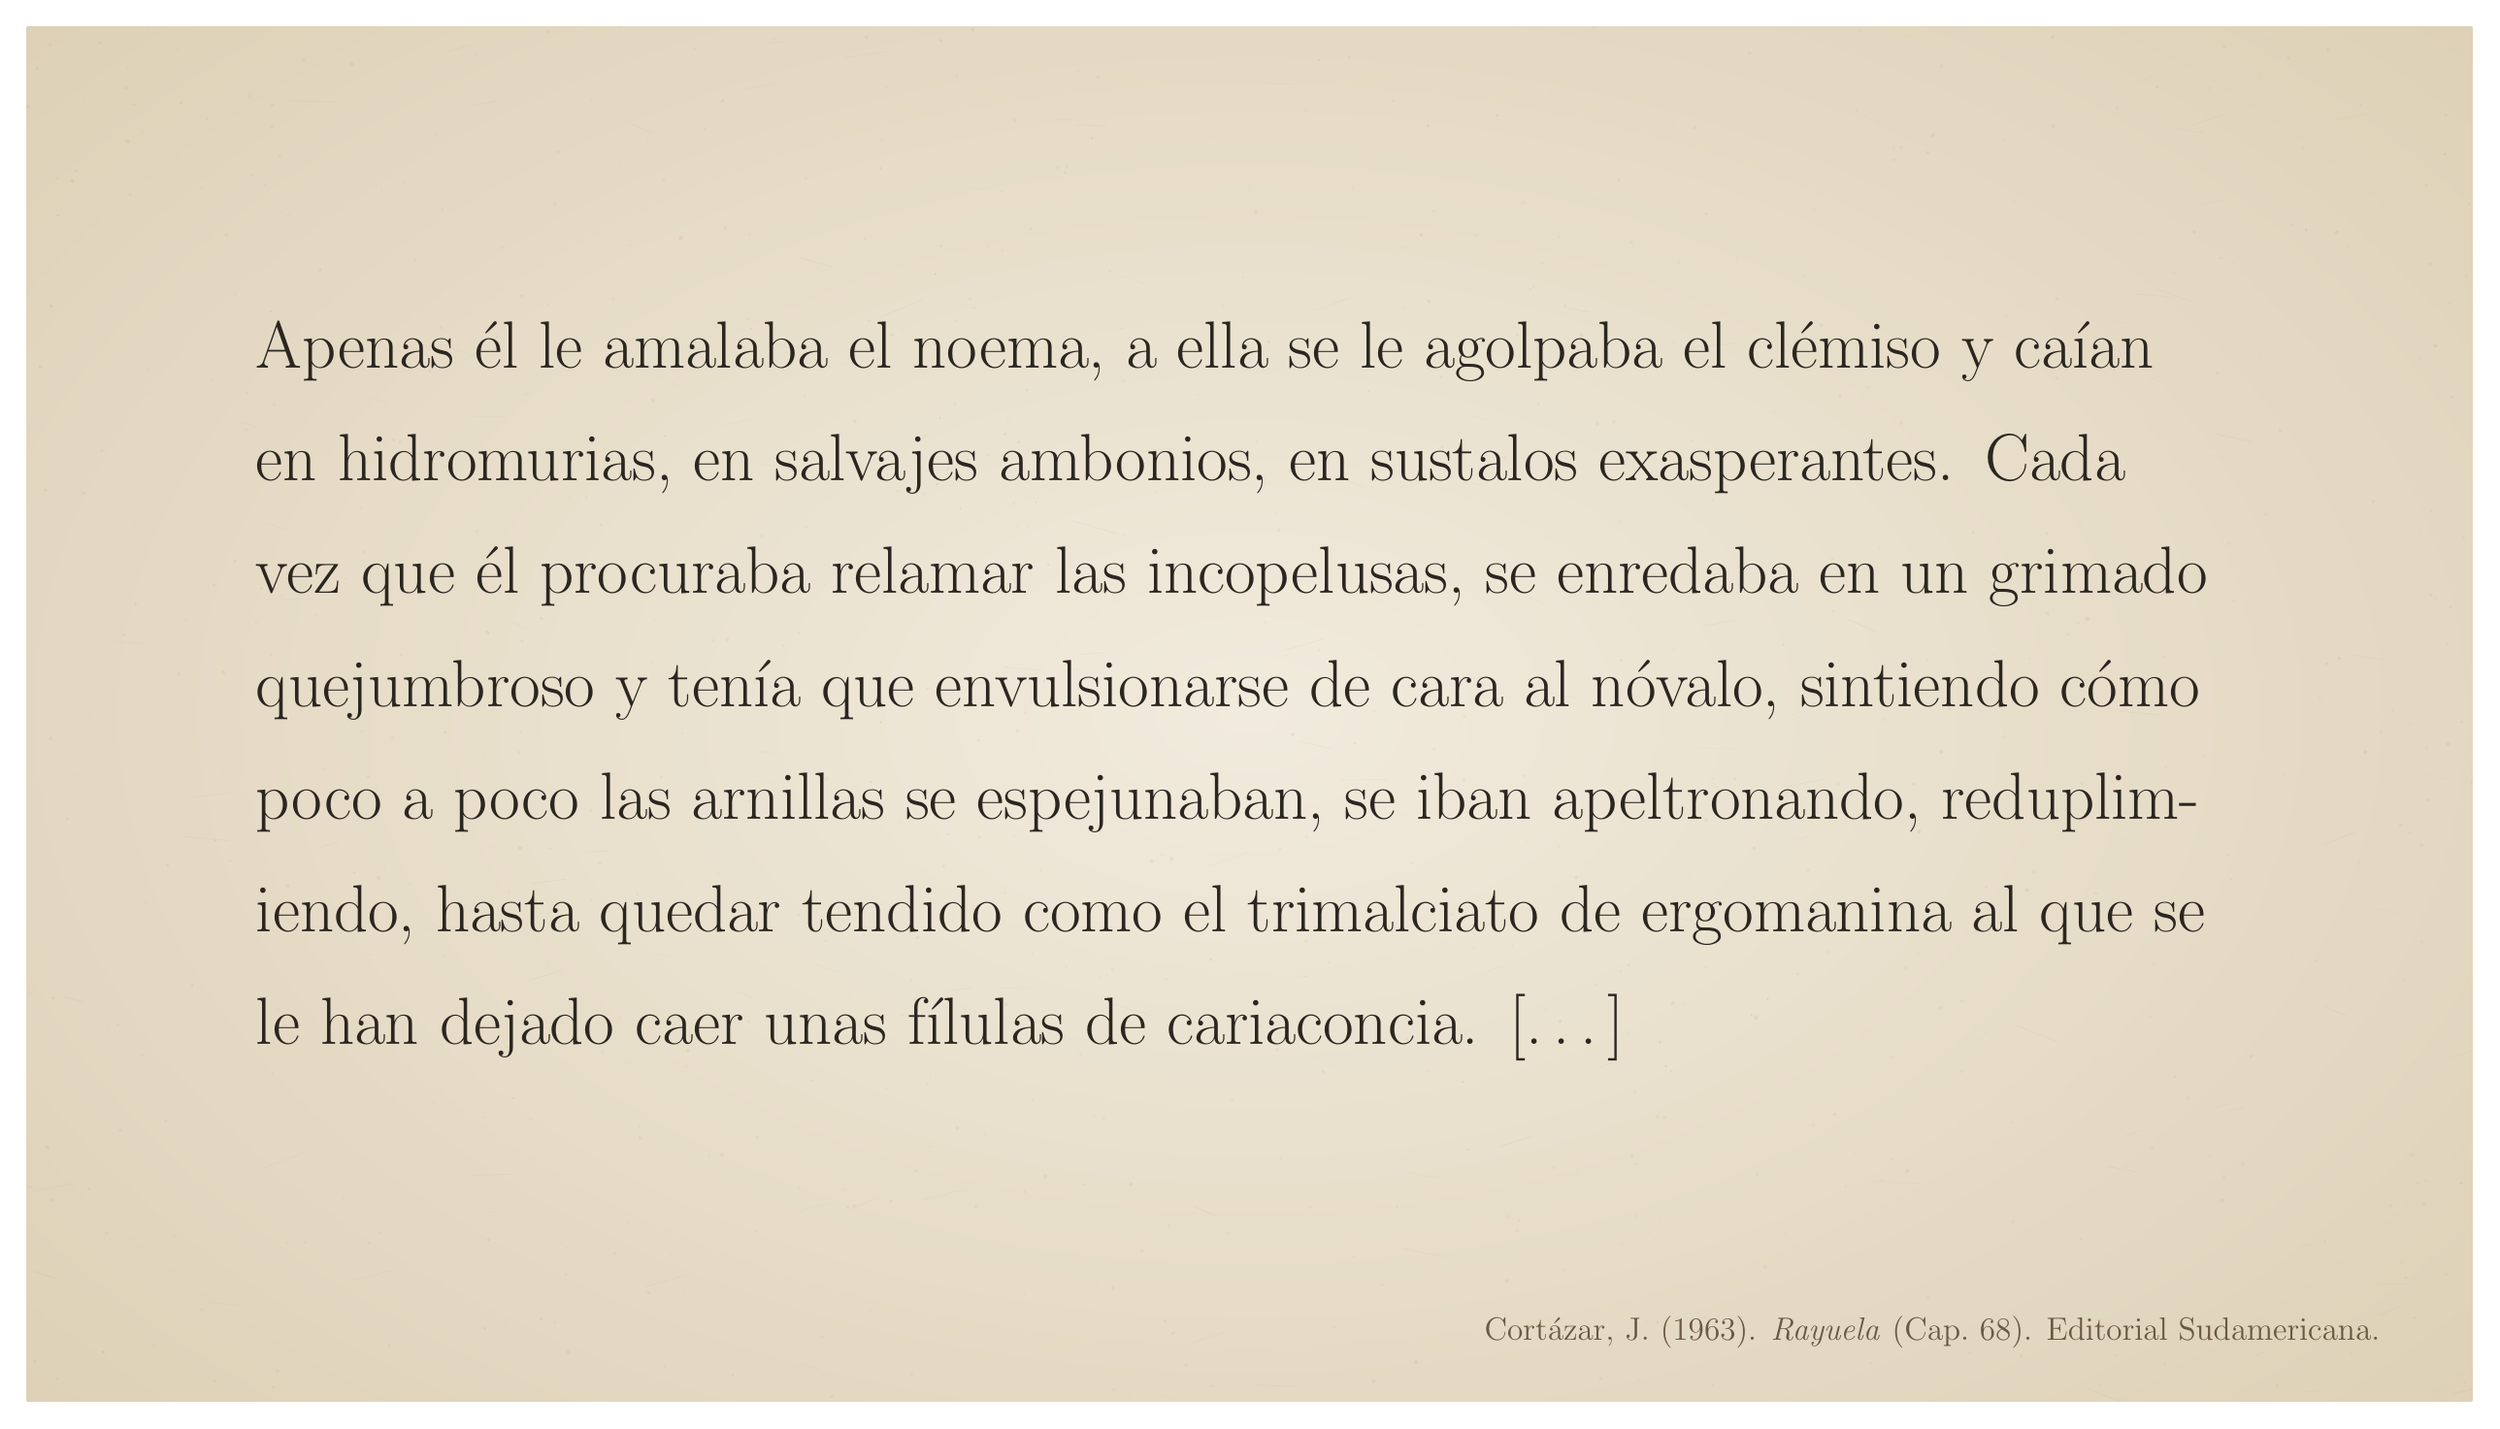
\begin{tikzpicture}
  \useasboundingbox (0,0) rectangle (\ancho,\alto);
  \clip (0,0) rectangle (\ancho,\alto);

  % Fondo con viñeta
  \fill[PergaminoBorde] (0,0) rectangle (\ancho,\alto);
  \shade[inner color=Pergamino, outer color=PergaminoBorde]
    (\ancho/2,\alto/2) ellipse [x radius=0.72*\ancho, y radius=0.80*\alto];

  % Textura (misma semilla que la Fase 1)
  \pgfmathsetseed{1914}
  \foreach \i in {1,...,900}{
    \pgfmathsetmacro{\x}{rnd*\ancho}
    \pgfmathsetmacro{\y}{rnd*\alto}
    \pgfmathsetmacro{\r}{0.008+0.02*rnd}
    \pgfmathsetmacro{\o}{0.05+0.12*rnd}
    \fill[Fibra, opacity=\o] (\x,\y) circle (\r);
  }
  \foreach \i in {1,...,140}{
    \pgfmathsetmacro{\x}{rnd*\ancho}
    \pgfmathsetmacro{\y}{rnd*\alto}
    \pgfmathsetmacro{\l}{0.15+0.5*rnd}
    \pgfmathsetmacro{\a}{-25+50*rnd}
    \pgfmathsetmacro{\o}{0.04+0.08*rnd}
    \draw[Fibra, opacity=\o, line width=0.25pt, rotate around={\a:(\x,\y)}]
      (\x,\y) -- ++(\l,0);
  }

  % Inicio del cap. 68 (gíglico)
  \node[text=Tinta, align=left, text width=\AnchoTexto cm, inner sep=0pt,
        font=\fontsize{\TamLetra}{\Interlinea}\selectfont]
    at (\ancho/2,\alto/2+0.3) {%
      Apenas él le amalaba el noema, a ella se le agolpaba el clémiso y caían
      en hidromurias, en salvajes ambonios, en sustalos exasperantes. Cada
      vez que él procuraba relamar las incopelusas, se enredaba en un grimado
      quejumbroso y tenía que envulsionarse de cara al nóvalo, sintiendo cómo
      poco a poco las arnillas se espejunaban, se iban apeltronando,
      reduplimiendo, hasta quedar tendido como el trimalciato de ergomanina
      al que se le han dejado caer unas fílulas de cariaconcia. […]%
    };

  % Referencia APA
  \node[anchor=south east, text=Referencia, inner sep=0pt,
        font=\fontsize{13}{16}\selectfont]
    at (\ancho-1.2,0.7)
    {Cortázar, J. (1963). \textit{Rayuela} (Cap.~68). Editorial Sudamericana.};
\end{tikzpicture}
\end{document}
